
\documentclass[oneside,intlimits,reqno]{scrbook}

\usepackage{array}
\usepackage{enumerate}
\usepackage{mathrsfs}
\usepackage{mathtools}
\usepackage{pgf,tikz}
\usetikzlibrary{arrows}
\usepackage{extarrows}
\usepackage{graphicx,makeidx}
\usepackage{a4wide}
\usepackage{ragged2e}
\usepackage[nottoc]{tocbibind}
\usepackage{amsmath,amssymb,amsthm,amsfonts}
\usepackage{mathabx}
\usepackage[utf8]{inputenc}
\usepackage[czech]{babel}
\usepackage{relsize}



\usepackage[unicode,breaklinks=true,hypertexnames=false]{hyperref}
\def\dotminus{\mathbin{\ooalign{\hss\raise1ex\hbox{.}\hss\cr
			\mathsurround=0pt$-$}}}
		
\usepackage[inline,attach]{asymptote}
\def\asydir{pictures/source}
\usepackage[dvips]{attachfile2}
%definice textu nad rovnítkem
\newcommand{\equal}[1]{\mathop{\overset{#1}{\resizebox{\widthof{.{\ensuremath{\mathop{\overset{#1}{\mathop{=}}}}.}}}{\heightof{=}}{$\mathop{=}$}}}}

%redefinice znaků
\renewcommand{\epsilon}{\varepsilon}
\let\crossedphi\phi
\renewcommand{\phi}{\varphi}
\renewcommand{\rho}{\varrho}
\renewcommand{\emptyset}{\font\cmsy = cmsy10 at 12pt\hbox{\cmsy \char 59}}


%definice českých uvozovek
\def\bq{\mbox{\kern.1ex\protect\raisebox{-1.3ex}[0pt][0pt]{''}\kern-.1ex}}
\def\eq{\mbox{\kern-.1ex``\kern.1ex}}
\gdef\uv#1{\bq #1\eq}


\renewcommand{\d}{\mathrm{d}} % diferenciál
\newcommand{\me}{\mathrm{e}} % eulerovo číslo
\newcommand{\E}{\mathbb{E}} % střední hodnota
\newcommand{\D}{\mathrm{D}} %  rozptyl
\newcommand{\LL}{\mathscr{L}}
\newcommand{\Loss}{\mathscr{L}}
\newcommand{\FF}{\mathrm{F}} % distribuční funkce
\newcommand{\PP}{\mathbb{P}} % pravděpodobnost
\newcommand{\NN}{\mathcal{N}}
\newcommand{\MSE}{\mathrm{MSE}}
\newcommand{\Exp}{\mathrm{Exp}}
\newcommand{\NF}{\mathrm{F}}
\newcommand{\AN}{\mathcal{AN}}
\newcommand{\sgn}{\mathrm{sgn}}
\newcommand{\A}{\mathrm{A}}
\newcommand{\BS}{\mathrm{BS}}
\newcommand{\HF}{H_F^{-1}}

\newcommand{\prostor}{(\Omega,\mathcal{A},\PP)} % prostor
\newcommand{\mi}{\mathrm{i}} % imaginární jednotka
\newcommand{\R}{\mathbb{R}} % množina reálných čísel
\renewcommand{\C}{\mathbb{C}} % množina komplexních čísel
\newcommand{\Z}{\mathbb{Z}} % množina celých čísel
\newcommand{\N}{\mathbb{N}} % množina přirozených čísel
\newcommand{\Cc}{\mathcal{C}} % funkce třídy C (spojité)
\newcommand{\I}{\textbf{I}} % identita
\newcommand{\Identita}[1]{\mathbb{I}_{#1}} % identita
\newcommand{\fisher}{\mathbb{I}} % Fisherova matice
\newcommand{\RR}{\mathcal{R}}
\newcommand{\RT}{\mathcal{R}_T}
\newcommand{\Be}{\mathrm{Be}}
\newcommand{\Bi}{\mathrm{Bi}}
\newcommand{\X}{\textbf{X}}
\newcommand{\Q}{\textbf{Q}}
\newcommand{\bt}{\boldsymbol{\theta}}
\newcommand{\bdelta}{\boldsymbol{\delta}}
\newcommand{\Y}{\textbf{Y}}

\newcommand{\PEX}{\PP^\X}
\newcommand{\fex}{f_\X}
\newcommand{\FEX}{\FF_\X}
\newcommand{\FT}{\FF_T}
\newcommand{\FR}{\lambda_T}
\newcommand{\CFR}{\Lambda_T}
\newcommand{\MRL}{\mathrm{MRL}}
\newcommand{\MTTF}{\mathrm{MTTF}}
\newcommand{\IFR}{\mathrm{IFR}}
\newcommand{\IFRA}{\mathrm{IFRA}}
\newcommand{\NBU}{\mathrm{NBU}}
\newcommand{\NBUE}{\mathrm{NBUE}}

\newcommand{\Weib}{\mathrm{Weib}}
\newcommand{\LN}{\mathcal{LN}}


\newcommand{\Aa}{\mathcal{A}}
\newcommand{\Bb}{\mathcal{B}}
\renewcommand{\t}{\theta} % theta
\newcommand{\bmu}{\boldsymbol{\mu}} % vektorové mí

\newcommand{\htm}{\widehat{\t}_\txt{M}}
\newcommand{\htb}{\widehat{\t}_\txt{B}}
\newcommand{\html}{\widehat{\t}_\txt{ML}}
\newcommand{\htn}{\widehat{\t}_n}
\newcommand{\rhn}{R_{H_0}}
\newcommand{\Phiast}{\crossedphi^\ast}
\newcommand{\rhno}{\overline{R}_{H_0}}
\newcommand{\freg}{\mathcal{F}_{reg}}
\newcommand{\fregp}{\mathcal{F}_{reg}^+}
\newcommand{\fregml}{\mathcal{F}_{reg}^\txt{ML}}
\newcommand{\fregmle}{\mathcal{F}_{reg}^\txt{MLE}}
\newcommand{\RE}{\mathrm{RE}_{2,1}}
\newcommand{\ARE}{\mathrm{ARE}_{2,1}}


%matematické výrazy
\newcommand{\tg}{\mathop{\mathrm{tg}}}
\newcommand{\argmin}{\mathop{\mathrm{argmin}}}
\newcommand{\argmax}{\mathop{\mathrm{argmax}}}
\newcommand{\argsup}{\mathop{\mathrm{argsup}}}
\renewcommand{\Re}{\mathop{\mathrm{Re}}}
\newcommand{\Ran}{\mathop{\mathrm{Ran}}}
\newcommand{\supp}{\mathop{\mathrm{supp}}}
\renewcommand{\Im}{\mathop{\mathrm{Im}}}
\newcommand{\Cov}{\mathbb{C}\mathrm{ov}}


%konvergence
\newcommand{\sj}{\stackrel{s.j.}{\longrightarrow}}
\newcommand{\Pto}{\stackrel{\PP}{\to}}
\newcommand{\wto}{\stackrel{w}{\to}}
\newcommand{\Dto}{\stackrel{\mathscr{D}}{\to}}
\newcommand{\PSJ}{\stackrel{\PP,s.j.}{\longrightarrow}}
\newcommand{\Lto}{\stackrel{(\mathscr{L})}{\to}}
\newcommand{\sjP}{\stackrel{s.j.~\PP}{\longrightarrow}}
\newcommand{\Lp}{\stackrel{L_p}{\longrightarrow}}

%nadtržítka
\newcommand{\overbar}[1]{\mkern 1mu\overline{\mkern-1mu#1\mkern-3mu}\mkern 3mu}
\newcommand{\Oxn}{\overbar{\rule{0ex}{1.8ex}X_n}}
\newcommand{\Oyn}{\overbar{\rule{0ex}{1.8ex}Y_n}}
\newcommand{\Ox}[1]{\overbar{\rule{0ex}{1.8ex}X_{#1}}}
\newcommand{\Oy}[1]{\overbar{\rule{0ex}{1.8ex}Y_{#1}}}
\newcommand{\oxn}{\overbar{\rule{0ex}{1.33ex}X_n}}
\newcommand{\ox}[1]{\overbar{\rule{0ex}{1.33ex}X_{#1}}}
\newcommand{\oy}[1]{\overbar{\rule{0ex}{1.33ex}Y_{#1}}}
\newcommand{\oyn}{\overbar{\rule{0ex}{1.33ex}Y_n}}
\newcommand{\omn}{\overbar{\rule{0ex}{1.3ex}\mu_n}}
\newcommand{\walpha}{\widehat{\alpha}}
\newcommand{\wbeta}{\widehat{\beta}}
\newcommand{\wgamma}{\widehat{\gamma}}

\newcommand{\hyn}{\widehat{y}_n}
\newcommand{\hyi}{\widehat{y}_i}
\newcommand{\hy}{\widehat{y}}
\newcommand{\lyn}{\overline{y}_n}
\newcommand{\ly}{\overline{y}}
\newcommand{\lhyn}{\overline{\hy}_n}
\newcommand{\lhy}{\overline{\hy}}
\newcommand{\lyi}{\overline{y}_i}
\newcommand{\RMR}{\mathrm{R}}
\newcommand{\SST}{\mathrm{SST}}
\newcommand{\SSE}{\mathrm{SSE}}
\newcommand{\SSR}{\mathrm{SSR}}
\newcommand{\lei}{\overline{e}_i}
\newcommand{\hei}{\widehat{e}_i}
\newcommand{\he}{\widehat{e}}
\newcommand{\Hobv}{\mathcal{H}_\text{obv}}
\newcommand{\HCF}{\mathcal{H}_\mathrm{CF}}
\newcommand{\RF}{\mathcal{R}}

\newcommand{\pB}{\widehat{p}_B}
\newcommand{\pML}{\widehat{p}_\mathrm{ML}}
\newcommand{\wmu}{\widehat{\mu}}

\newcommand{\TV}{\mathrm{TV}}
\newcommand{\Ev}{\mathrm{Ev}}
\newcommand{\Dd}{\mathscr{D}}
\newcommand{\Rr}{\mathscr{R}}

\newcommand{\oxnn}{\overbar{\rule{0ex}{1.33ex}x_n}}

%stříšky
\newcommand{\hsn}{\widehat{\sigma}_n^2}

%posloupnosti
\newcommand{\posl}{(X_j)_{j=1}^{+\infty}}
\newcommand{\poslkon}{(X_j)_{j=1}^{n}}
\newcommand{\posln}{(X_n)_{n=1}^{+\infty}}
\newcommand{\poslnn}{(\X_n)_{n=1}^{+\infty}}

%sumy
\newcommand{\suminftyo}{\sum\limits_{n=0}^{+\infty}}
\newcommand{\suminfty}{\sum\limits_{n=1}^{+\infty}}
\newcommand{\sumainfty}[1]{\sum\limits_{#1}^{+\infty}}
\newcommand{\suminftylo}{\sum\limits_{l=0}^{+\infty}}
\newcommand{\sumin}{\sum\limits_{i=1}^{n}}
\newcommand{\sumjn}{\sum\limits_{j=1}^{n}}
\newcommand{\sm}[2]{\sum\limits_{ #1 }^{ #2 }}


\newcommand{\dom}[1]{\mathop{\mathrm{Dom} (#1)}} % definiční obor
\newcommand{\mat}[1]{\mathbf #1}
\newcommand{\abs}[1]{\left|#1\right|}
\renewcommand{\b}[1]{\left( #1 \right)}
\newcommand{\nor}[1]{\left\|#1\right\|}
\newcommand{\Br}[1]{\Bigl(#1\Bigr)}
\newcommand{\br}[1]{\bigl(#1\bigr)}
\newcommand{\e}[1]{\me^{#1}}
\newcommand{\inv}[1]{#1^{-1}}
\newcommand{\ini}{\theta\in\Theta}
\newcommand{\init}[1]{\theta\in\Theta\subset\R^#1}

\newcommand{\txt}[1]{\mathrm{{\footnotesize  #1 }}}
\newcommand{\matice}[4]{\left(\begin{array}{cc}	#1 & #2 \\ #3 & #4	\end{array} \right)}
\newcommand{\maticehrana}[4]{\left[\begin{array}{cc}	#1 & #2 \\ #3 & #4	\end{array} \right]}
\newcommand{\vektor}[2]{\left(\begin{array}{c}	#1  \\  #2	\end{array} \right)}
\newcommand{\p}[1]{\PP\left( #1 \right)}
\newcommand{\EE}[1]{\E\left[ #1 \right]}
\newcommand{\n}[1]{\NN\left( #1 \right)}
\newcommand{\hypothesis}[2]{H_0: #1 ~\text{vs.}~ H_1: #2 }
\newcommand{\hypothesiswide}[2]{H_0: #1 \qquad\text{vs.}\qquad H_1: #2 }
\newcommand{\silofunkce}[1]{\beta_\crossedphi\big|_{\Theta_{#1}}}
\newcommand{\silofunkceast}[1]{\beta_{\Phiast}\big|_{\Theta_{#1}}}
\newcommand{\hypothesisap}[2]{H'_0: #1 ~\text{vs.}~H'_1: #2 }
\newcommand{\test}[1]{\boxed{\text{TEST: $H_0$ zamítáme, pokud } #1 .}}
\renewcommand{\S}{\mathbb{S}}


% Prostředí
\theoremstyle{definition}
\newtheorem{define}{Definice}[chapter]
\theoremstyle{plain}
\newtheorem{theorem}[define]{Věta}
\newtheorem{lemma}[define]{Lemma}
\newtheorem{dusl}[define]{Důsledek}
\newtheorem{corollary}[define]{Tvrzení}
\renewcommand{\proofname}{Důkaz}

\theoremstyle{remark}
\newtheorem{example}[define]{\textsc{Příklad}}
\newtheorem{remark}[define]{\textsc{Poznámka}}

\renewcommand{\indexname}{Rejstřík}


\usepackage[symbol]{footmisc} %Speciálná \footnote{}
\renewcommand{\thefootnote}{\fnsymbol{footnote}}

\usepackage[makeroom]{cancel} %pokrácení ve zlomku

\usepackage{placeins} %\FloatBarrier

\usepackage{pdfpages} %scan

\frenchspacing
\setlength{\parindent}{0pt}
\setlength{\parskip}{1.5pt}
\setlength{\headheight}{10pt}
\setlength{\headsep}{12pt}
\setlength{\textheight}{690pt}
\setlength{\footskip}{15pt}

\hypersetup{
 	pdftitle={01SKEMEU - Příručka ke státnicím},
 	pdfauthor={Martin Kovanda},
 	pdfsubject={Zápisky z přednášek SKE a MEU, FJFI ČVUT},
 	pdfkeywords={Spolehlivost a extrémní události},
 	bookmarksnumbered=true,
 	colorlinks=true,
 	pdfpagemode={UseOutlines}
 }
\makeindex

\title{01SKE + 01MEU}
\date{\today}
\author{01SKE: Bc. Martin Kovanda \& Bc. Jakub Bureš \\ 01MEU: \\  \\
	dle přednášek Ing. Václava Kůse, Ph.D.}

\begin{document}

% ****************************************************************************************************************************
%                             FRONTMATTER
% ****************************************************************************************************************************
\frontmatter
\maketitle

\newpage
\pdfbookmark[0]{Obsah}{obsah}
\tableofcontents

\chapter*{Předmluva a poděkování}
\pdfbookmark[0]{Předmluva}{predmluva}

Materiál byl sestaven na~základě online přednášek a~prezentací Ing. Václava Kůse, Ph.D. Zmíněné přednášky proběhly v~letním semestru akademického roku 2020/2021 na~Fakultě jaderné a fyzikálně inženýrské ČVUT v~Praze. Přednášky nebyly uskutečněny prezenční formou vzhledem k~probíhající pandemii Covid-19.
\\ \\
Doufám, že Vám tato příručka usnadní studium těchto předmětů a dostatečně Vás namotivuje k jejich absolvování u státnic. Tato příručka vynechává veškeré důkazy a v mnoha oblastech je zjednodušující. Je nicméně dělána tak, aby v ní bylo vysvětleno vše, co je potřeba k pochopení problematiky a k úspěšnému absolvování státnicového předmětu. Pro lepší pochopení předmětů je silně doporučeno navštívit přednášky.
\\ \\
Toto skriptum je určeno studentům navazujícího magisterského studia navštěvujícím předměty 01SKE\emph{ Spolehlivost systémů a klinické experimenty} a 01MEU\emph{ Modelování extrémních událostí}, které jsou zařazeny mezi státnicové předměty oboru AMSM. Při~sestavování textu se~předpokládaly znalosti matematiky na~úrovni kurzů 01MAB2-4, 01LAB1-2, 01MIP a~01MAS.



% ****************************************************************************************************************************
%                             MAINMATTER
% ****************************************************************************************************************************
\mainmatter
\chapter{[SKE] Spolehlivostní charakteristiky, obecné rodiny hustot, cenzorování, bayesovské odhady v analýze spolehlivosti.}

Budeme pracovat s veličinou  $0\leq T\sim \FT$, která reprezentuje čas do poruchy (\textbf{Failure Time}), třeba do první chyby nebo do uzdravení pacienta. Více se však pracuje s $\RT(t)=1-\FT(t)=\PP(T>t)$ jakožto \textbf{Reliability Function}. Střední doba života (\textbf{Mean Time to Failure}) je vypočtena jako $$\MTTF:=\E T=\int_{0}^{+\infty}\big(1-\FT(t)\big)\d t - \int_{-\infty}^0\FT(t)\d t = \int_{0}^{+\infty}\RT(t)\d t=:\mu.$$

\begin{define}
	\textbf{Mediánový život} $t_\mathrm{med}$ je definován jako $\RT(t_\mathrm{med})=\frac{1}{2}$ a  \textbf{pravý krajní bod} $t_\FF$ jako  $t_\FF=\inf\{ t:\FT(t)\geq1 \}$ ($\RT$ v tomto bodě skočí na nulu a už je dále nula).
\end{define}

\begin{define}
	Intenzitu poruch (FR - \textbf{Failure Rate}) se definuje jako  $\FR(t)=\frac{f_T(t)}{\RT(t)}$.
\end{define}

Význam této veličiny je (úpravou definice) $\FR(t)=\lim\limits_{\Delta t\to 0+}\frac{1}{\Delta t}\PP(t<T\leq t+\Delta t|T>t)$, tedy že výrobek přežil do času $t$ a v následujícím $\Delta t$ čase se pokazí. Tato veličina se definuje, protože je lépe uchopitelná. Může být rostoucí i klesající. Funkce $\RT(t)$ naproti tomu je vždy klesající a pohybuje se v intervalu $[0,1]$.

\begin{theorem}[Vztahy] Platí, že
	$$ \FR(t)=\frac{-\RT(t)}{\RT(t)}=-\frac{\d}{\d t}\big(-\ln \RT(t)\big). $$
	Definujeme \textbf{Cumulative Failure Rate} jako $\Lambda_T(t):= -\ln\RT(t)$. Potom
	$$ \CFR(t) = \int_{0}^{t}\FR(u)\d u. $$
	Dále platí, že 
	$ 1-\FT(t)=\RT(t)=\e{-\CFR(t)} = \e{-\int_{0}^{t}\FR(u)\d u}$. Celkově tedy existuje jednoznačný vztah mezi $\FT$ a $\FR$ za předpokladu spojité distribuční funkce.
\end{theorem}

\begin{figure}[h]
	\centering    
	\begin{tikzpicture}
	\node[inner sep=0pt,anchor=north west] (pic) at (0,0)
	{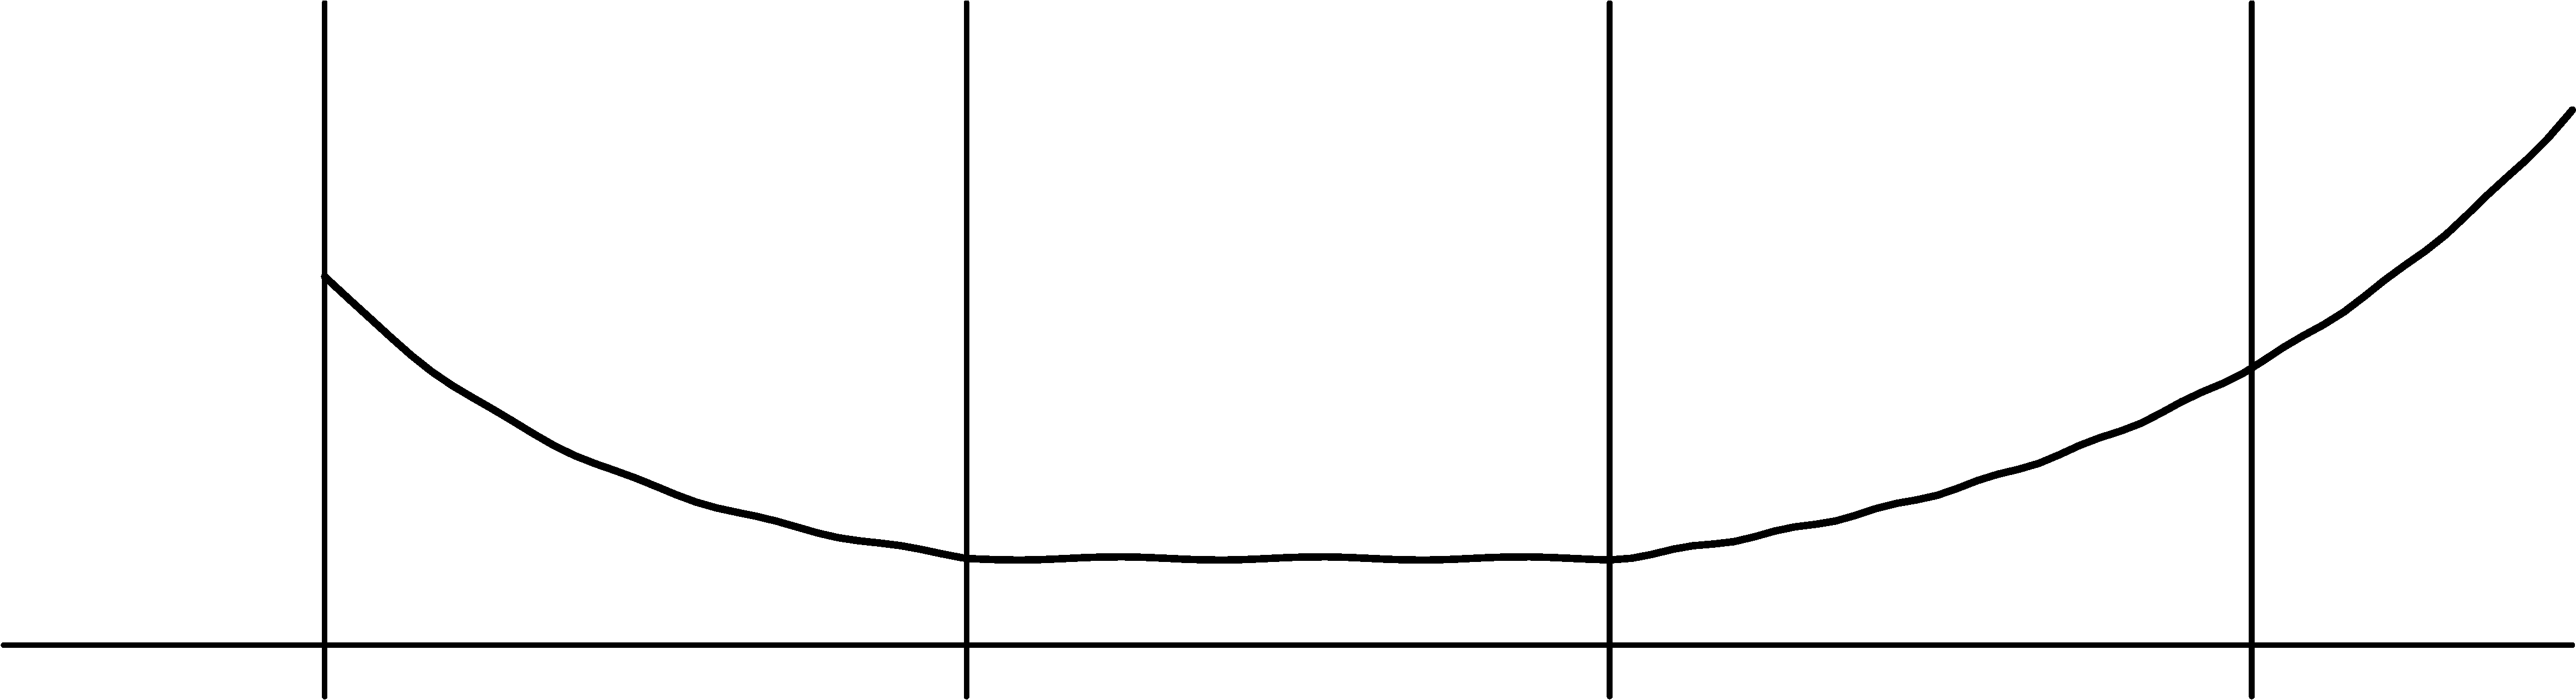
\includegraphics[width=10cm]{pictures/faze.pdf}};
	\draw [color=black](2.36,-0.2) node[anchor=north west] {I};
	\draw [color=black](4.76,-0.2) node[anchor=north west] {II};
	\draw [color=black](7.17,-0.2) node[anchor=north west] {III};
	\draw [color=black](1.3,-1.95) node[anchor=north west] {zajíždění};
	\draw [color=black](3.82,-1) node[anchor=north west] {fáze běžného};
	\draw [color=black](3.82,-1.5) node[anchor=north west] {provozu};
	\draw [color=black](7,-1.95) node[anchor=north west] {stárnutí};
	\draw [color=blue!50!black](0.72,-2.5) node[anchor=north west] {$0$};
	\draw [color=blue!50!black](9.1,-2.5) node[anchor=north west] {$t$};
	\draw [color=blue!50!black](9.2,-1) node[anchor=north west] {$\FR(t)$};
	\end{tikzpicture}
	\caption{Klasický průběh intenzity poruch (technické výrobky apod.).} \label{faze}
\end{figure}

Klasický výrobek se chová podle obr. \ref{faze}. V první fázi se vylaďují výrobní vady, a proto intenzita klesá. Ve druhé fázi je intenzita víceméně konstantní (běžný provoz). V závěrečné fázi materiál stárne a intenzita se zvyšuje.

\begin{define}
Pro $t>0$ definujeme $\RR(x|t):=\PP(T>t+x|T>t)=\frac{\RT(t+x)}{\RT(t)}$ jako \textbf{podmíněná spolehlivost}.	
\end{define}

\begin{define}
Definujeme \textbf{mean residual life} jako $$\MRL(t)=\mu(t)=\int_{0}^{+\infty}\RR(x|t)\d x=\frac{1}{\RT(t)}\int_{t}^{+\infty}\RT(u)\d u.$$
\end{define}

\begin{define}
	Pro $t_2>t_1>0$ definujeme $\RR(t_1,t_2):=\PP(T>t_2|T>t_1)$ jako \textbf{intervalovou spolehlivost}.
\end{define}

\section{Rodiny spolehlivostních modelů}
\begin{define}
	Zavádíme rodinu spolehlivostních modelů \textbf{IFR} (Increasing FR) s rostoucí FR, pokud $\FR(t)$ je rostoucí. Obecněji (pokud by nebyla k dispozici hustota) pak pokud je $\CFR$ konvexní.
	
	Analogicky naopak zavádíme \textbf{DFR} (Decreasing FR).
\end{define}

\begin{define}
	Distribuje $\FF$ je z \textbf{IFRA} rodiny (Increasing RF in Average), pokud $\frac{\CFR(t)}{t}$ je funkce rostoucí na $t>0$.
	
	Analogicky \textbf{DFRA} pro funkci klesající na $t>0$, případně $t\in(0,\t_\FF)$.
\end{define}

\begin{define}
	$\FF$ je z třídy \textbf{NBU} (New Better than Used), pokud $\RR(x|t)\leq\RR(x)=\RR(x|t=0)$, $\forall t>0,\forall x>0$. Analogicky \textbf{NWU} jako New Worse than Used.
\end{define}

\begin{define}
		$\FF$ je z třídy \textbf{NBUE} (New Better than Used in Expectation), pokud $\MRL(t)\leq \MTTF(t)$, $\forall t>0$. Analogicky \textbf{NWUE}.
\end{define}

\begin{theorem}
	$\IFR\Rightarrow\IFRA\Rightarrow\NBU\Rightarrow\NBUE$.
\end{theorem}

\section{Cenzorovaná data}
Doteď se pracovalo s úplným výběrem. Měli jsme tedy $n$ $iid$ objektů a pozorovaly se všechny časy do poruchy. Nyní se však pracuje s živými objekty (lidmi, zvířaty apod.), které se mohou rozhodnout pozorování opustit. Může se například cenzorovat časem, tj. experiment se ukončí po nějakém čase. Může se cenzorovat i počtem poruch, tj. experiment je ukončen po $r$-té poruše. Třetí možností je cenzorovat náhodně. Každý pocient je tedy cenzorován jeho vlastním cenzorovaným časem, což je náhodná veličina s $\FF_C$.

\begin{example}
	Exponenciální rozdělení $T\sim\Exp(\lambda)$ má následující vlastnosti:\begin{enumerate}
		\item $f_T(t)=\lambda\e{-\lambda t}$, $\RT(t)=\e{-\lambda t}$, $\CFR=\lambda t$, $\RR(x|t)=\e{-\lambda t}$, $\FR(t)=\lambda$
		\item $\MTTF=\frac{1}{\lambda}$, $\MRL(t)=\MTTF$
		\item celkově tedy IFR=DFR, IFRA=DFRA, NBU=NWU
	\end{enumerate}
\end{example}
\begin{theorem}[Smirnoffova transformace]
	Mějme čas do poruchy $T\sim\RT$, $\widetilde{T}:=\CFR(T)=-\ln\RT(T)$. Pak $\widetilde{T}\sim\Exp(1)$ s $\lambda_{\widetilde{T}}=1$ konstantní (tedy nestárne, ani nemládne, což vyplývá z vlastností exponenciálního času do poruchy). Navíc platí, že $T=t\Leftrightarrow \widetilde{T}=\CFR(t),~\forall t>0$ (pro spojité modely).
\end{theorem}

\section{Bayesovské odhady v analýze spolehlivosti}

\begin{define}[Gamma rozdělení]
	Mějme $T|\lambda\sim \Exp(\lambda)$ u nestabilní výroby ($\lambda=\lambda(t)$). Zde se vyplatí použít nějaké apriorní informace o $\lambda$, tedy $\lambda\sim\pi(\lambda)=\mathrm{Gamma}(k,\beta)$. Potom
	$$ \RT(t)=\int_{t}^{+\infty}f_T(u)\d u=\int_{t}^{+\infty}\int_{0}^{+\infty}\Exp(\lambda)\mathrm{Gamma}(k,\beta)\d\lambda\d u =\int_{0}^{+\infty}\mathrm{Gamma}(k,\beta)\RR_{T|\lambda}(t)\d\lambda=\frac{\beta^k}{(\beta+t)^k}, $$
	což je Paretovo rozdělení (s těžkým chvostem). Dále platí, že $\FR(t)=\frac{k}{\beta+t}$, což je klesající funkce, takže se toto rozdělení hodí např. pro modelování první fáze výrobku.
\end{define}

\begin{example}
	Jiná možnost by byla pro $(T_1...T_n)~iid~T|\lambda\sim\Exp(\lambda)$, $\lambda\sim\mathrm{Gamma}(k,\beta)$ odhadnout parametr $\lambda$ bayesovsky a dosadit ji do $\E T|\lambda$. Parametry $(k, \beta)$ lze nalézt např. pomocí empirického Bayese.
\end{example}

% lecture 5
	Užitečná je metoda pro life-time aplikace. Například k lékaři chodí v různém čase různí pacienti, takže se nabízí možnost vzít první sadu pacientů, odhadnout na ní nějaký parametr a postupně tento parametr updatujeme dalšími sadami pacientů.

Dejme tomu, že chceme udělat predikci pro $T_{n+1}$ čas do poruchy za předpokladu, že máme data $\textbf{t}=(t_1,...,t_n)$. Potom Bayesovská prediktivní spolehlivost $R_{T_{n+1}}(t):=\PP\big(T_{n+1}>t\big| t_1,...,t_n\big)=\int_{t}^{+\infty}f_\mathrm{B}^{\mathrm{PR}}(t)\d t$ se vypočítá na základě Bayesovské prediktivní hustoty ve tvaru $f_\mathrm{B}^{\mathrm{PR}}(t):=\int_{0}^{+\infty}f_T(t|\theta)\pi(\theta|\textbf{t})\d\t$. Tento způsob je sice komplikovaný, ale třeba pro měnící se $\lambda$ nejsou jiné metody k dispozici.
\chapter{[SKE] Parametrické modely s (ne)monotónní intenzitou poruch, únavové cyklické zkoušky, příklady použití.}

\begin{define}[Normální rozdělení]
	Mějme $T\sim \NN(\mu, \sigma^2)$ (kde zanedbáme zápornou část, tedy chceme $\mu$ dostatečně daleko od nuly). Platí, že 
	$$ \FR(t)=\frac{\frac{1}{\sigma}\phi\big(\frac{t-\mu}{\sigma}\big)}{1-\Phi\big(\frac{t-\mu}{\sigma}\big)}.$$
		Dále se může použít useknuté normální rozdělené v $t=0$ zleva $\mathcal{TN}(\mu,\sigma^2)$, tedy $$\RT(t)=\frac{\PP(T>t)}{\PP(T>0)}=\frac{1-\Phi\big(\frac{t-\mu}{\sigma}\big)}{1-\Phi\big(\frac{\mu}{\sigma}\big)}.$$ Pro $t>0$ je $\FR(t)$ shodná s předešlým případem.
\end{define}

Normální rozdělení se tedy dá použít na modelování třetí fáze opotřebování výrobku.

\begin{define}[Gamma rozdělení]
Mějme $T_i\sim \Exp(\lambda)$. Pak $T:=\sum_{1}^{k}T_j$ je čekací doba na výskyt $k$-té poruchy (třeba pokud máme $k$ náhradních dílů). Tím dostáváme $T\sim\mathrm{Gamma}(k,\lambda)$. $\lambda>0$ nazýváme \textbf{intenzita šoků} a $k>0$ míru rezistence. Víme dále, že $\MTTF=\E T=\frac{k}{\lambda}$. 
\end{define}

\begin{define}[Weibulovo rozdělení]
	Definujeme \textbf{Weibulovo} rozdělení definováno vztahem $\RT(t)=\e{-(\lambda t)^\alpha}$, tedy $f_T(t)=\alpha \lambda^\alpha t^{\alpha-1}\e{-(\lambda t)^\alpha}$. Platí, že
	$$ \FR(t)=\alpha\lambda^\alpha t^{\alpha-1},~\MTTF=\frac{1}{\lambda}\Gamma\big(1+\frac{1}{\lambda}\big),~t_\mathrm{med}=\frac{1}{\lambda}(\ln2)^{1/\alpha}.$$
\end{define}

\begin{theorem}[Reprodukce pro minimum]
	Mějme $(T_i)_{i=1}^n~iid~\Weib(\alpha,\lambda_j)$, $\forall j$. Potom platí, že 
	$$ T_s:=\min(T_i)_{i=1}^n \sim \Weib\big(\alpha,\left\|\boldsymbol{\lambda}\right\|\big)\equal{\lambda_j=\lambda}\Weib\big(\alpha,\lambda n^{1/\alpha}\big).$$
\end{theorem}

Toto se velice hodí na sériové systémy, protože systém je vyřazen při pokažení libovolné části systému (třeba zapojení žárovek).

\begin{define}[Lognormální rozdělení]
	Platí, že $T\sim \LN(\mu,\sigma^2)~\Leftrightarrow~\ln T\sim\NN(\mu,\sigma^2)$. Dále platí, že $$\RT(t)=\PP(T>t)=\PP(\ln T>\ln t)=\PP\Big(\frac{\ln T-\mu}{\sigma}>\frac{\ln T-\mu}{\sigma}\Big)=1-\Phi\Big(\frac{\ln T-\mu}{\sigma}\Big),$$ tedy $f_T(t)=\frac{1}{\sqrt{2\pi}\sigma t}\e{-\frac{1}{2\sigma^2}(\ln t-\mu)^2}$, vše pro $t>0$.
\end{define}

Dále platí, že $t_\mathrm{med}=\e{\mu}$, $\MTTF=\e{\mu+\frac{\sigma^2}{2}}$, $t_\mathrm{mod}=\e{\mu-\sigma^2}$ a $\D T=\e{2\mu}\big(\e{2\sigma^2}-\e{\sigma^2}\big)$. Pro FR (ponecháno čtenáři) platí, že $\lim\limits_{t\to+\infty}\FR(t)=0$.

Tento model se dá použít jako doba do opravy, nebo u cyklických trhacích zkoušek.

\subsection{Únavové zkoušky materiálu}
Při těchto zkouškách jde o to, aby se např. vyzkoušel materiál před tím, než je použitý na nějaký výrobek. Tento materiál se upne do trhacího přístroje a nechá se posílat do materiálu sílu nějakým cyklickým způsobem, např. sinusoidní síla $F_s=s\sin(\phi t)$. Při různé amplitudě $s$ (stresor) se materiál chová jinak, při nějaké se neděje nic, při nějaké se materiál může roztrhnout. Označme $N$ jako počet cyklů do rozlomení materiálu. Tato veličina je výrazně propojena z časem do poruchy $T=M\cdot\delta t$. Průběh může být třeba i lognormální, při výrobě můžou vzniknout vady a ty můžou součástku roztrhnout. Po nějaké době se však všechny tyto vady projeví a intenzita poruch začíná klesat (bohužel až k nule, ale stačí to k aproximaci).

Fyzikální opodstatnění spočívá v tom, že $Ns^b=c$, kde $b$ a $c$ jsou konstanty, které závisí na daném materiálu (geometrie, složení apod.). Po zlogaritmování dostaneme lineární vztah (k lineární regresi)
$$ \ln N=\ln c-b\ln s + \epsilon, $$
protože $\ln N\sim \NN$.


\begin{define}[Birnbaum-Sanders (BS) rozdělení]
	 Mějme $n$ únavových cyklů se zatížením $s$. Částečné poškození součástky po $i$-tém cyklu nazveme $Z_i$. Předpokládejme, že $Z_1,...,Z_n~id/iid\sim \big(\mu(s),\sigma^2(s)\big)$. Označme celkové poškození jako $W_n=\sumin Z_i$ a kritickou hranici poškození jako $w$ (poté se materiál roztrhne). Platí, že 
	 $$ \PP(N\leq n)\sim \PP(W_n>w)=1-\PP\big(\sumin Z_i\leq w\big)\equal{CLT}1-\PP\Big(\frac{\sumin Z_i-n\mu}{\sqrt{n}\sigma}\leq \frac{w-n\mu}{\sqrt{n}\sigma}\Big)=1-\Phi\Big(\frac{w-n\mu}{\sqrt{n}\sigma}\Big). $$
	 Přejděme nyní k $N\leftrightarrow T$ a $n\leftrightarrow t$. Dostaneme tím 
	 $$ \PP(T\leq t)=1-\Phi\Big(\frac{w-t\mu}{\sqrt{n}\sigma}\Big)=1-\Phi\Big(\frac{1}{\alpha}\big(\frac{1}{\sqrt{\lambda t}}-\sqrt{\lambda t}\big)\Big), $$ kde $\alpha=\frac{\sigma}{\sqrt{\mu w}}>0$ a $\lambda=\frac{\mu}{w}>0$. Potom $\RT(t)=\Phi\Big(\frac{1}{\alpha}\big(\frac{1}{\sqrt{\lambda t}}-\sqrt{\lambda t}\big)\Big)$, což je spolehlivost $\BS(\lambda,\alpha)$ rozdělení. Můžeme také vypočítat $f_T(t)=C\e{-\frac{1}{2\alpha^2}\big(\sqrt{\lambda t}-\frac{1}{\sqrt{\lambda t}}\big)^2}$, takže má trochu těžší chvosty, než normální rozdělení (ale menší, než lognormální rozdělení). Dále $\D T=\frac{\alpha^2}{\lambda^2}\Big(1+\frac{5\alpha^2}{4}\Big)$.
\end{define}

% lec 5

\subsection{Neparametrické metody}
Mějme nyní $T\sim\FT$, data $\textbf{t}=(t_1,...,t_n)$ a tedy uspořádaný výběr $\big(t_{(1)},...,t_{(n)}\big)$. Z toho můžeme udělat odhady $\overline{t_n}$, $\widehat{t_\mathrm{med}}$, $\hsn$, výběrový koeficient variace $\widehat{\mathrm{CV}}=\frac{s_n}{|\overline{t_n}|}$ a výběrovou disperzi $\widehat{\mathrm{CV}}^2$. Výběrový koeficient variace se dá využít třeba k detekci exponenciálního modelu ($\mathrm{CV}=1$) apod.

Dále můžeme získat empirickou spolehlivostní funkci $R_n(t)$, všechny vlastnosti jako nestrannost, konzistenci, AN apod. se přenáší z distribuční funkce.

Často se ještě používá modifikace empirické spolehlivostní funkce se jménem Crowderův plot, který vynese dvojice $\big\{t_{(j)}, \overline{R_n}\big(t_{(j)}\big)\}_{j=0}^n$, kde $t_{(0)}=0$ a $\overline{R_n}\big(t_{(0)}\big)=1$ a $\overline{R_n}\big(t_{(j)}\big)=\frac{R_n\big(t_{(j)}\big)+R_n\big(t_{(j)-}\big)}{2}$ (funkce připomíná klesající schody, kde skoky jsou nahrazeny prostředním bodem). Použití nalezneme třeba v porovnání $\overline{R_n}$ s Weibulovým rozdělením a můžeme se podívat, jak si dané křivky odpovídají.

Dále se může použít například Weibull Probability Plot. Pokud totiž $T\sim\Weib(\lambda,\alpha)$, pak $\RT(t)=\e{-(\lambda t)^\alpha}$, tedy $\ln\big(-\ln R(t)\big)=\alpha\ln\lambda+\alpha\ln t$. Potom se nabízí udělat Crowderův plot, tedy $\ln t$ oproti $\ln\big(-\ln R(t)\big)$ je přímka, pokud sedí Weibulovský model. Můžeme tedy definovat WPP plot pro data $\textbf{t}$ jako $\big\{\ln t_{(j)},\ln\big(-\ln \overline{R}(t_{(j)})\big)\}_1^n$. Pokud se skutečně ukáže lineární závislost, pak je Weibull dobrý kandidát na spolehlivostní model.


\chapter{[SKE] Spolehlivost komponentních systémů, redundantní struktury, důležitost komponent.}

% lecture 7
\section{Komponentní systémy}
    \begin{define}
        Předpokládejme, že máme systém o $n$ komponentách. Budeme charakterizovat stav $i$-té komponenty $x_i$ binárně jako funguje/nefunguje, tedy $x_i\in\{0,1\}$. Označme $\textbf{x}=(x_1,...,x_n)$ jako \textbf{stavový vektor}. 
        
        Předpokládejme, že známe-li $\textbf{x}$, pak známe stav celého systému $S$, tzn. jsme schopni definovat \textbf{strukturní funkci} $\crossedphi(\textbf{x})=\begin{cases}
        1,&\text{systém funguje,}\\0,&\text{systém nefunguje.}
        \end{cases}$
    \end{define}

    Tímto způsobem můžeme zkoumat různě zapojené součásti, třeba sériově, 
    paralelně (jsou tedy v redundanci) apod. U sériového zapojení stačí 
    jedna vadná součástka, aby systém přestal fungovat a u paralelního 
    systému stačí, když alespoň jedna součástka funguje, aby systém 
    fungoval. Pozor ale, že záleží na reprezentaci, někdy se např. sériově 
    zapojené součástky chovají, jako by byly paralelní (např. ventily na 
    potrubí, aby voda netekla, alespoň jeden ventil musí fungovat).

    \begin{corollary}
        Logické zapojení komponent se může zakreslit pomocí blokových diagramů (RBD - Reliability Block Diagram) (podobné elektrickému zapojení). Pro sériově zapojené součásti máme 
        $$ \crossedphi(\textbf{x})=\prod_{i=1}^{n}x_i=\min(x_i)_1^n.$$
        Paralelně zapojené součástky pak
        $$ \crossedphi(\textbf{x})=1-\prod_{i=1}^{n}(1-x_i)\equal{ozn}\bigsqcup_{i=1}^n x_i=\max(x_i)_1^n, $$ kde $\bigsqcup$ označuje inverzní produkt.
    \end{corollary}

    \begin{define}[k-o-o-n struktura]
        k-o-o-n struktura (k-out-of-n) je taková, že systém funguje, pokud je alespoň $k$ z komponent je funkční. Potom
        $$ \crossedphi(\textbf{x})=\begin{cases}
        1,&\text{pokud }\sumin x_i\geq k,\\0,& \text{jinak.}
        \end{cases}$$
        Tento systém se může použít třeba pro přivolávání hasičů, pokud 2oon zaznamenají kouř. Tímto se eliminují false positive chyby ve stylu zapálená cigareta apod. Například systém 2oo3 se dá zapsat jako paralelní vlákna $\{(1,2), (2,3),(1,3)\}$. Není to však jediná možnost, viz obrázek \ref{fig:2oo3}.
        
        \begin{figure}[h]
            \centering
            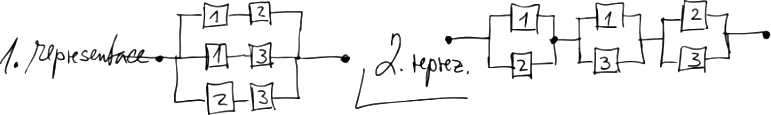
\includegraphics[width=0.7\linewidth]{pictures/2oo3}
            \caption{Dvě možnosti zapojení systému 2oo3, paralelní systém minimálnních cest (vlevo) a série minimálních řezů (vpravo).}
            \label{fig:2oo3}
        \end{figure}
        
        Máme tedy $\crossedphi(\textbf{x})=x_1x_2\bigsqcup x_1x_3\bigsqcup x_2x_3$
    \end{define}

    \begin{theorem}
        Mějme systém S o $n$ komponentech. Mějme dále minimální cesty $P_1,...,P_k$ (funkční cesty ze kterých nelze nic odstranit). Pak $$ \crossedphi(\textbf{x})=\bigsqcup_{j=1}^k \prod_{i\in P_j} x_i.$$
        Naopak z minimálních řezů $K_1,...,K_l$ můžeme dostat
        $$ \crossedphi(\textbf{x})= \prod_{j=1}^k \bigsqcup_{i\in K_k} x_i.$$
        V praxi pak používáme ten vzorec, který nejvíce zjednodušuje výpočet.
    \end{theorem}

    \begin{corollary}
        Definujeme strukturu BRIDGE (viz obr. \ref{fig:bridge}). Tady máme 4 cesty, kudy projít, tedy $\{(1,2),(4,5),(1,3,5),(4,3,2)\}$. Z toho můžeme udělat $\crossedphi(\textbf{x})$. Poměrně jednoduše se dá udělat i diagram řezů.
        
        \begin{figure}[h]
            \centering
            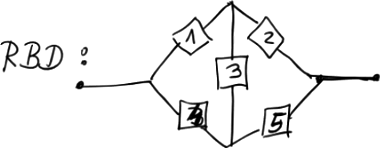
\includegraphics[width=0.3\linewidth]{pictures/bridge}
            \caption{Strukture BRIDGE.}
            \label{fig:bridge}
        \end{figure}
        
    \end{corollary}

    \begin{theorem}[Pivotální rozklad]
        Mějme systém $S$ o $n$ komponentách. Pak můžeme $\crossedphi(\textbf{x})$ rozepsat jako 
        $$\crossedphi(\textbf{x})=x_i\crossedphi(1_i,\textbf{x}_{-i})+(1-x_i)\crossedphi(0_i,\textbf{x}_{-i}),$$
        kde fixujeme, že $i$-tý prvek funguje/nefunguje. Tento rozklad se může použít rekurentně až do 
        $$\crossedphi(\textbf{x})=\sum_{\textbf{y}}\prod_{j=1}^n x_j^{y_j}(1-x_j)^{1-y_j}\crossedphi(\textbf{y}),$$ kde $\textbf{y}$ jsou $n$-rozměrné binární vektory, kterých je $2^n$.
    \end{theorem}

    Toto se hodí např. pro BRIDGE, kde je ideální udělat rozklad podle prvku 3. Potom dostaneme 
    $$ \crossedphi(\textbf{x})=x_3\crossedphi(1_3,\textbf{x}_{-3})+(1-x_3)\crossedphi(0_3,\textbf{x}_{-3}). $$ 
    Tím se výrazně zjednoduší struktura systému.

    \begin{define}[Strukturní důležitost komponent]
        Stavový vektor $(1_i,\textbf{x})$ se nazývá \textbf{kritická cesta/vektor pro $i$-tou komponentu}, pokud $\crossedphi(1_i,\textbf{x})=1\wedge \crossedphi(0_i,\textbf{x})=0 $, tzn. $\crossedphi(1_i,\textbf{x})-\crossedphi(0_i,\textbf{x})=1$.
        
        Označme $\eta_\crossedphi(i)=\sum_{(\cdot_i,\textbf{x}_{-i})} \big[\crossedphi(1_i,\textbf{x})-\crossedphi(0_i,\textbf{x})\big]$ počet kritických vektorů pro $i$-tou komponentu.
        
        Číslo $B_\crossedphi(i)=\frac{\eta_\crossedphi(i)}{2^{n-1}}$ nazveme \textbf{Birmbaumova míra (strukturní) důležitosti} $i$-té komponenty v $S$.
    \end{define}

    \begin{example}
        Komponenta 1 je v sérii s paralelní 2 a 3. Pak pro $i=1$ dostaneme
        $$\begin{array}{c|c}
            (\cdot,x_2,x_3) & \crossedphi(1_i,\textbf{x})-\crossedphi(0_i,\textbf{x})=1 \\\hline
            \cdot\,00 & 0 \\
            \cdot\,01 & 1 \\
            \cdot\,10 & 1 \\
            \cdot\,11 & 1 
        \end{array}.$$
        Jelikož $2^{n-1}=4$, pak $\eta_\crossedphi(1)=3$, takže $B_\crossedphi(1)=\frac{3}{4}$ apod.
        
    \end{example}


    \begin{define}
        $i$-tá komponenta se nazývá \textbf{irelevantní}, pokud $\crossedphi(1_i,\textbf{x})=\crossedphi(0_i,\textbf{x})$, $\forall\textbf{x}_{-i}$. Tedy že na jejím vypnutí/zapnutí nezáleží. Příkladem je záznamové zařízení při požárním poplachu, které je sice důležité, ale na samotný poplach nemá vliv.
    \end{define}

    \begin{define}
        Systém komponent se nazývá \textbf{koherentní}, pokud neobsahuje irelevantní komponenty a strukturní funkce je neklesající v každé své proměnné.
    \end{define}

    \begin{theorem}
        Pro $S$ koherentní platí, že $\crossedphi(\textbf{0})=0$, $\crossedphi(\textbf{1})=1$ a $$ \prod_{i=1}^n x_i\leq \crossedphi(\textbf{x})\leq \bigsqcup_{i=1}^n x_i. $$
    \end{theorem}

    \begin{define}[Spolehlivostní funkce]
        Pro výpočet $R_S(t)$ využijeme čas $t$ a ztotožníme poruchovostní komponenty 
        $$X_i(t)=\begin{cases}1,&\text{s pravděpodobností }p_i=\PP(T_i>t),\\0,&\text{jinak.}\end{cases}$$
        Dosazením do strukturní funkce potom vyrobíme $\crossedphi\big(\textbf{X}(t)\big)$, kde $\textbf{X}(t)$ je vektor veličin $X_i(t)$, které charakterizují funkčnost/nefunkčnost komponenty v čase $t$. Potom
        $$ R_S(t)=\PP(T_S>t)=\PP\big(\crossedphi\big(\textbf{X}(t)\big)=1\big)=1\cdot\PP\big(\crossedphi\big(\textbf{X}(t)\big)=1\big)+0\cdot\PP\big(\crossedphi\big(\textbf{X}(t)\big)=0\big)=\EE{\crossedphi\big(\textbf{X}(t)\big)}. $$
    \end{define}

    \begin{example}
        Pro sériově zapojený $S$ dostaneme
        $$ R_S(t)=\E \crossedphi\big(\textbf{X}(t)\big)\equal{id}\prod_{i=1}^n \E X_i(t)=\prod_{i=1}^n R_i(t)=\prod_{i=1}^n \e{-\int_{0}^{t}\lambda_i(\tilde{t})\d\tilde{t}}=\e{-\int\limits_{0}^t\sumin \lambda_i(\tilde{t})\d\tilde{t}}, $$
        kde $\sumin \lambda_i(\tilde{t})\d\tilde{t}=\lambda_S(\tilde{t})$. Z toho vyplývá, že např. pro 100 komponent o $R_i(t)=0.995$ dostaneme systém o spolehlivosti $R_s(t)=0.606$. Sériové systémy jsou tedy nejhorší možné, co se týče spolehlivosti. 
    \end{example}

    \begin{example}
        Pomocí tří imaginárních komponent (DFR,CFR,IFR) jde modelovat fyzická (reálná) komponenta s vanovitým průběhem FR. U paralelních součástí máme naopak 
        $$ R_S(t)=\E\crossedphi\big(\textbf{X}(t)\big)=\E\Big[\bigsqcup_{i=1}^n X_i(t)\Big]=\E\Big[1-\prod_{i=1}^n(1-X_i(t))\Big]\equal{id}1-\prod_{i=1}\big(1-R_i(t)\big)=\bigsqcup_{i=1}^n R_i(t). $$
    \end{example}

    \begin{example}
    S je k-o-o-n: 
    $$ R_S(t)=\E\crossedphi\big(\textbf{X}(t)\big)= \PP\big(\sum_{i=1}^n X_i(t)\geq k\big)\equal{iid}\sum_{x=k}^n {n\choose x} R(t)^{x} (1-R(t))^{n-x} = \sum_{x=k}^n {n\choose x} \e{-\lambda tx} \big(1-\e{-\lambda t}\big)^{n-x}   $$
    Z čehož můžeme potom získat střední dobu do poruchy
    $$\MTTF_S = \sum_{x=k}^n {n\choose x} \int_0^\infty \e{-\lambda tx} \big(1-\e{-\lambda t}\big)^{n-x} \d t = \Bigg| \e{-\lambda t} = y \Bigg| = \dots =  \frac{1}{\lambda} \sum_{x=k}^n \frac{1}{x},$$
    kde jsme využili substice, která integrál převede na beta funkci a dále se dá zjednodušit do výše uvedeného tvaru. V tabulce jsou uvedeny konkrétní případy $\MTTF$ pro různá $k$ či $n$.

    \begin{table}[h]
        \centering
        \begin{tabular}{|l|l|l|l|l|}
            \hline
            $k$\textbackslash $n$& 1 & 2 &3  & 4 \\ \hline\hline
            1&$\frac{1}{\lambda}$  &  $\frac{3}{2}$$\frac{1}{\lambda}$& $\frac{11}{6}$$\frac{1}{\lambda}$ & $\frac{25}{12}$$\frac{1}{\lambda}$ \\ \hline
            2& $\times$ & $\frac{1}{2}$$\frac{1}{\lambda}$ & $\frac{5}{6}$$\frac{1}{\lambda}$ &  \\ \hline
            3&  &  & $\frac{1}{3}$$\frac{1}{\lambda}$ &  \\ \hline
            4&  &  &  & $\frac{1}{4}$$\frac{1}{\lambda}$ \\ \hline
        \end{tabular}
    \end{table}
    \end{example}

\section{Redundance}

    \begin{theorem}
        Mějme $n$-komponentní systém $S$ a stavové vektory $\textbf{x}$, $\textbf{y}$. Potom pro koherentní strukturu S platí $\crossedphi(\textbf{x} \bigsqcup \textbf{y}) \geq  \crossedphi(\textbf{x}) \bigsqcup \crossedphi(\textbf{y})$.
    \end{theorem}

%lecture 9

    V této úloze řešíme, jakým způsobem lze uchopit zálohu nějaké části systému.

    \subsection*{Aktvní záloha}
    
    Aktivní záloha je pararelní záloha části systému a je v plném provozu a může se tedy porouchat. Tyto systémy json obyčejné paralelní systémy, které jsme doposud dělali. Můžeme tedy spočítat $R_S$, $\lambda_S$, $\MTTF_S$, apod.
    
    \subsection*{Pasivní záloha + perfect switch}
    
    Rezervní komponenta čeká ve stand-by režimu a její rozbití v tomto čase zanedbáme. V této úloze máme switch, který musí být schopný zařadit do systému rezervní komponentu.
    Pokud počítáme s perfektně fungujícím switchem, potom se dá vypočítat $T_S = \sum_{i=1}^n T_i$, $\MTTF = \sum_{i=1}^n \MTTF_i$, $R_S(t) = \PP\Big(\sum_{i=1}^n T_i\Big) = \otimes_{i=1}^n R_i(t)$ a pro dostatečně velké $n$ je $\sum_{i=1}^n T_i $ asymptoticky normální nebo $AG_{\alpha}$.
    
    \subsection*{Pasivní záloha + imperfect switch}
        Zde charakterizujeme switch pomocí pravděpodobnosti, tedy pravděpodobnost, že switch skutečně přepne na záložní komponentu, je 1-$p$. 
        Předpokládáme navíc, že komponenty včetně switche jsou nezávisle fungující. Mohou nastat 2 případy.
            \begin{enumerate}
                \item Komponenta 1 drží až do času t, to nastane s pravděpodobností $R_1(t)$.
                \item Komponenta 1 se porouchala v určitém čase v $(0,t)$, když označíme $\tau < t$ jako čas poruchy,tak se komponenta 1 porouchala v $(\tau,\tau + \d\tau)$. Pravděpodobnost, že nastane tato situace se dá jednoduše zapsat jako hustota $f_{T_1}(\tau)\d\tau$ $\longrightarrow$ Switch přepne s pravděpodobností 1-$p$ v čase $\tau$ $\longrightarrow$ Komponenta 2 je nyní aktivní v čase $\tau$ a funguje až do $t$. Toto nastane s pravděpodobností $R_2(t-\tau)$.
            \end{enumerate}
    Podívejme se nyní na pravděpodobnost, že je celý tento systém $S$ funkční. Platí, že
    \begin{align*}
        \PP\big(\text{ je OK v čase }t \big) =  & \PP(T_S > t ) = R_S(t) = \PP(\mathrm{i.}) + \PP(\mathrm{ii.}) = \\ &
        R_1(t) + \int_0^t (1-p)R_2(t-\tau) f_{T_1}(\tau)\d\tau = \\ &
        \e{-\lambda_1 t} + \int_0^t (1-p)\e{-\lambda_2 (t-\tau)} \lambda_1\e{-\lambda_1 \tau}  \d\tau = \\ &
        \e{-\lambda_1 t} + \frac{(1-p)\lambda_1}{\lambda_1-\lambda2}\e{-\lambda_2 t} - \frac{(1-p)\lambda_1}{\lambda_1-\lambda2}\e{-\lambda_1 t}.
    \end{align*}
    Navíc můžeme také určit 
    \begin{align*}
        \MTTF_S = \int_0^{\infty} R_S(t) \d t = \frac{1}{\lambda_1} + \frac{1-p}{\lambda_2}.
    \end{align*}

    \subsection*{Částečná záloha + imperfect switch}
    
    Rezervní komponenta je pod minimálním zatížením a může se tedy porouchat.  Máme $T_1$ se spolehlivostí $R_1$, $T_2$ se spolehlivostí $R_2$ a switch, který přepíná s pravděpodobností $(1-p)$. Navíc máme $T_0 \sim R_0$, což je doba do poruchy komponenty 2 v době minimálního zatížení. Obdobně lze rozdělit na dva případy.
    \begin{enumerate}
        \item Komponenta 1 drží až do času t, to nastane s pravděpodobností $R_1(t)$.
        \item Komponenta 1 se porouchala v určitém čase v $(0,t)$, když označíme $\tau < t$ jako čas poruchy,tak se komponenta 1 porouchala v $(\tau,\tau + \d\tau)$. Pravděpodobnost, že nastane tato situace se dá jednoduše zapsat jako hustota $f_{T_1}(\tau)\d\tau$ $\longrightarrow$ Switch přepne s pravděpodobností 1-$p$ v čase $\tau$ $\longrightarrow$ Komponenta 2 není porouchána v čase $\tau$, nastává s pravděpodobností $R_0(\tau)$ $\longrightarrow$ Komponenta 2 je funkční v čase $t$, tzn. $R_2(t-\tau)$.
    \end{enumerate}
    
    Máme tudíž o jednu variantu navíc, než v předchozím případě. Opět lze určit 
    \begin{align*}
        R_S(t) = &	R_1(t) + \int_0^t (1-p)R_0(\tau)R_2(t-\tau) f_{T_1}(\tau)\d\tau = \\ &
        \e{-\lambda_1 t} + \frac{(1-p)\lambda_1}{\lambda_0+\lambda_1-\lambda_2}\big(\e{-\lambda_2 t} - \e{-(\lambda_0 + \lambda_1) t} \big)
    \end{align*}
    a
    \begin{align*}
        \MTTF_S = \int_0^{\infty} R_S(t) \d t = \frac{1}{\lambda_1} + \frac{1-p}{\lambda_2} - (1-p)\frac{\lambda_0}{\lambda_2(\lambda_1 + \lambda_0)}.
    \end{align*}
    
\section{Extreme Value Distribution (EVD)}

    V této části budeme pořítat spolehlivost pro extrémní události. Budeme tedy zkoumat, jak jsou rozloženy minima a maxima nějaké iid posloupnosti pozorování. To ale přesně odpovídá tomu, co se probíralo v minulých sekcích pro sériové a paralelní systémy.

    \begin{define}[Gumbelovo rozdělení (sériový systém)]
        Nechť $T_j \sim f_T(t) = o\big(\e{-\beta\abs{t}} \big)$ (exponenciální chvosty) při $t \rightarrow \infty$, ale není useknuté zleva (např. Gauss, ale ne Pareto). Pak 
        $$ U_n:=\min(T_j)_1^n  \Dto Y  ,$$ kde
        pro distribuční funkci náhodné veličiny $Y$ platí, že	
        $$ \FF_Y(t)  = 1 - \e{-\exp(\frac{t-\vartheta}{\alpha} )},~~t \in \R, \vartheta \in \R, \alpha \in\R^+,  $$
        což se nazývá \textbf{Gumbelovo rozdělení} (extreme value distribution type 1).
    \end{define}
    
    Toto rozdělení se hodí pro modelování III části pro výrobky, kde je možné předpokládat dokonce exponenciální nárůst intenzity poruch. Takovéto výrobky spadají také do tzv. Gompertz-Makehamova zákona. Ten říká, že pravděpodobnost smrti roste exponenciálně s věkem.

    \begin{define}[Gumbelovo rozdělení (paralelní systém)]
        Nechť $T_j \sim f_T(t) = o\big(\e{-\beta\abs{t}} \big)$ (exponenciální chvosty) při $t \rightarrow \infty$, ale není useknuté zprava (prakticky vždy vyhovuje ). Pak 
        $$ M_n:=\max(T_j)_1^n  \Dto Y  ,$$ kde
        pro distribuční funkci náhodné veličiny $Y$ platí, že	
        $$ \FF_Y(t)  = \e{-\exp(-\frac{t-\vartheta}{\alpha} )},~~t \in \R, \vartheta \in \R, \alpha \in\R^+,  $$
        což se nazývá \textbf{Gumbelovo rozdělení} pro maximum.
    \end{define}
    

\chapter{[SKE] Odhady spolehlivosti a kumulativní intenzity poruch, typy cenzorování, testy.}
%lecture 10

    \subsection*{Model konkurenčních rizik (Competing risks)}
    
    V této části budeme uvažovat vícero typů poruch $\delta \in \lbrace1,2,\dots k \rbrace$. Nechť je $T$ doba do poruchy. Můžeme si to představit jako sériové zapojení $k$ rizik, které soutěží o vyřazení komponenty, proto Competing risks. To má širokou škálu využití v praxi, $T$ může být například doba trvání manželství, které může končit z mnoha příčin. V ekonomii se může jednat o dobu do krachu firmy. Ve stavitelství se můžeme bavit o době do pádu určitého mostu, apod.
    
    Máme tedy dvojce $(T_j, \delta_j)_{j=1}^n$, $T_j \geq 0$ a $\delta_j\in\widehat{k}$, kde $T_j$ i $\delta_j$ jsou náhodnými veličinami. V ideálních datech pro vyhodnocování by měly být zastoupeny všechny možnosti poruch, jinak není možné takový systém modelovat. Každá dvojce má sdruženou distribuční funkci $(T_j, \delta_j) \sim \FF_{T,\delta}(t,d)$, kde $t\in\R, d\in \R$. Tato distribuční funkce je ovšem v $d$ diskrétní, čili v proměnné $d$ se nachází skoky. Nyní $\FF_{T,\delta}(t,d)$ charakterizujme pomocí subdistribucí
    $$R(t,j) := \PP(T > t, j),\quad t \in \R,~j \in \widehat{k},$$ 
    $$p_j = \PP(\delta = j) = R(0,j),\quad\sum_{i=1}^k p_i = 1.$$ 
    Budeme potřebovat také subhustoty, které definujeme jako $f(t,j)=-R'(t,j)$. Pomocí tohoto objektu lze určit hustota marginální hustota pro $T$, či distribuční a spolehlivostní funkce. Platí tedy, že
    $$f_T(t) = \sum_{i = 1}^{n}f(t,j),\quad\text{a tedy}\qquad\FF_T(t) = \int_{-\infty}^{t} \sum_{j=1}^n f(y,j)\d y = \sum_{j=1}^n \FF(t,j).  $$
    Dále lze odvodit
    $$R_T(t) = \int_{t}^{\infty} \FF(y,j) \d y = \sum_{j=1}^n R(t,j),\qquad r_T(t) = \frac{f_T}{R_T} = \sum_{j=1}^n\frac{f(t,j)}{R_T} = \sum_{j=1}^n r_T(t,j). $$
    Můžeme definovat také relativní intenzitu poruch $j$-tého módu rizika $\frac{r_T(t,j)}{r_T(t)}$.
    Pokračujme definováním dalších veličin,
    $$ R_T(t|j) := \PP(T > t|\delta =j) = \frac{\PP(T > t, \delta =j)}{\PP(\delta =j)} = \frac{R(t,j)}{p_j}, $$
    $$R_T(t) = \sum_{j=1}R(t,j) = \sum_{j=1}p_j R_T(t|j).$$
    V poslední rovnosti jsme získali $R_T(t)$ jako konvexní směs podmíněných distribucí. Tyto vztahy platí i v případě, že jednotlivé módy rizika jsou na sobě závislé.

\section{LIFE-TIME aplikace}

    Budeme využívat \emph{Censoring} dat. To lze udělat několika způsoby.

    \paragraph{Censorování typu I.} Experiment ukončíme v čace $t_c$. Data jsou tvaru $T_{(1)},T_{(2)},\dots, T_{(r)} \leq t_c$, přičemž máme informaci, že $T_{(r+1)},T_{(r+2)},\dots, T_{(n)} > t_c$. To lze zapsat i jako
    $$W_j := \min(T_j,t_c), \quad \delta_j = I\lbrace T_j \leq t_c \rbrace \in\{0,1\}.$$
    Tato úloha by šla řešit přes konkurenční rizika, ale byl by to overkill. V následující větě se podíváme jak se dá sestrojit vztah pro hustotu pravděpodobnosti prvních $r$ uspořádaných statistik, včetně $r$, které je náhodné.
    
    \begin{theorem}
        Nechť $T_1, T_2, \dots, T_n$ jsou iid $\FF$ (nebo $f$). Označme $T_{(1)} < T_{(2)} < \cdots <T_{(r)}$, kde $r\in\widehat{n}$. Pak 
        $$f(t_{(1)}, t_{(2)}, \dots, t_{(n)}, r) = \frac{n!}{(n-r)!}\Big(\prod_{j=1}^r f(t_{(j)})\Big)R(t_c)^{n-r}, \quad  \forall t_{(1)} < t_{(2)} < \cdots <t_{(r)} \leq t_c $$ 
        a navíc
        $$f(t_{(1)}, t_{(2)}, \dots, t_{(n)} |r) = \frac{r!}{\FF^r(t_c)}\prod_{j=1}^r f(t_{(j)}) = r! \prod_{j=1}^r  \frac{f(t_{(j)})}{\FF(t_{c})}, \quad  t_{(j)} \leq t_c,$$ 
        což se dá interpretovat jako useknutá hupsti, která je proto přenormovaná hodnotou $\FF(t_{c})$.
    \end{theorem}

    \paragraph{Censorování typu II.}
    Také se jinak nazývá censorování poruchou. V tomto typu censoringu volíme $r$ pevně a čas experimentu (zde označme $t_{\mathrm{exp}} = t_{(r)}$) je náhodná veličina. Data pak vypadají takto: 
    $$W_j = \min(T_j, t_{(r)})_{j=1}^n,\quad \delta_j = I\lbrace T_j \leq t_{(r)} \rbrace \in \{0,1\}. $$
    I zde můžeme formulovat podobnou větu, jako v případě Censoringu typu I.
    
    \begin{theorem}
        Nechť $T_1, T_2, \dots, T_n$ jsou iid $\FF$ (nebo $f$). Označme $T_{(1)} < T_{(2)} < \cdots <T_{(r)}$, kde $r\in\widehat{n}$. 
        Pak $$f(t_{(1)}, t_{(2)}, \dots, t_{(n)}, r) = \frac{n!}{(n-r)!}\Big(\prod_{j=1}^r f(t_{(j)})\Big)R(t_{(r)})^{n-r}, \quad  \forall t_{(1)} < t_{(2)} < \cdots <t_{(r)} \leq t_c. $$ 
    \end{theorem}
    
    \paragraph{Censorování typu III.}
    
    Kombinace přechozích dvou censorování, tedy nastavíme pevně čas experimentu $t_c$ a také nastavíme pevně $r$. Potom bereme to, co přijde dříve, jestli $r$ poruch, nebo jestli dojde čas.
    
    \paragraph{Random censoring, RC.}
    Máme opět čas do poruchy $T\sim\FF_T$, navíc máme ovšem další náhodnou veličinu $C\sim\FF_C$, kterou nazveme časový cenzor. Obě tyto veličiny jsou vzájemně nezávislé. Časový cenzor realizuje censorování každé jednotlivé časové hodnoty. Data v tomto případě zapisujeme ve tvaru
    $$W = \min(T,C), \quad \delta = I\lbrace T \leq C \rbrace. $$
    Tím dostáváme opět spojitě diskrétní rozdělení pro dvojici
    $(W,\delta)$ v modelu konkurenčních rizik. Tím máme hotový setup modelu. Střední hodnotu potom můžeme vypočítat jako
    $$q = \EE{\delta} =  \EE{I\lbrace T \leq C \rbrace} = \int\limits_{\lbrace T \leq C \rbrace}1\d\PP = \PP(T\leq C)\equal{id} \iint_{t\leq c}\d\FF_T\d\FF_C = \iint_{t\leq c}f_Tf_C  \d t \d c.$$
    Víme-li, že máme k dispozici $n$ pozorování, potom číslo $n\cdot q$ značí střední počet poruch v $n$-tici opakování. \\
    Zaznamenáváme $T_j, C_j$, což vede na data ve tvaru $(W_j,\delta_j)_{j=1}^n$. Dále označme $D$ množinu indexů, kdy opravdu došlo k poruše, čili $$D = \lbrace j\in \widehat{n}: \delta_j =1 \rbrace .$$ Často nazývána také jako množina defektů. Mohutnost množiny $\abs{D} = \# D = \delta = \sum_{j=1}^n\delta_j$, tedy počet poruch v $n$-tici. 
    
    \begin{remark}
        Spolehlivostní funkci $R_T(t)$ v klinických testech většinou značíme jako $S_T(t)$ a je známa pod názvem Survival function. 	
    \end{remark} 
    
    \paragraph{Random censoring zleva.}
    Představme si situaci, kdy doktor musí určit diagnózu, sleduje pacienty, přičemž při již probíhajících testech přijde další pacient. Doktor ho tudíž nesleduje od úplného začátku, ale sleduje ho až od nějakého času $t_{l}$. Někdy známo také jako oboustranné censorování.
    
    \paragraph{RC + censoring typu I.}
    Pracujeme ze živými objekty, které můžou být censorované, ovšem může se stát, že na experiment není dostatek času nebo financí a tudíž musí být experiment ukončen v pevném čase $t_{c}$. Je to tedy smíšené censorování.
    
    \begin{remark}[RC s neúplnou informací.]
    Jedná se o běžný RC, avšak nedokážeme zaznamenat poruchu v tom čase, kdy skutečně nastala. O poruše se dozvíme až na konci celého experimentu. Například pacient onemocnění, ale nepřijde k doktorovi, porucha tudíž skutečně nastala, ale pacient ji neoznámí. Po skončení experimentu doktor obvolá pacienty, že se končí s experiemntem a až v tom okamžiku se pacient přizná, že onemocněl.\\
    Máme tedy jistou pravděpodobnost $p$, že porucha nebyla zachycena a je dostupná až po skončení po experimentu.
    \end{remark}
    
    \section{Výpočty v RC modelech.}
    Začneme větou, která nám prozradí, jak vypadá sdružená hustota veličiny $(W, \delta)$.
    \begin{theorem}
        $W$ je náhodná veličina vzhledem k běžné spojité Lebesgueově míře $\lambda$ a náhodná veličina $\delta$ je náhodná veličina vzhledem k čítací míře $\kappa$. Dále jsou $T$ a $C$ nezávislé, přičemž máme k dispozici $f_T$ a $f_C$. Pak platí
        $$f(w,\delta) =  \Big[f_T(w)(1-F_C(w))\Big] ^{\delta}\Big[f_C(w)(1-F_T(w)) \Big]^{1-\delta}$$
        pro $\forall \delta\in\lbrace 0,1\rbrace$ a $\forall w\in\R^{+}$ vzhledem k součinové míře $\lambda \times \kappa$.
    \end{theorem}

    \begin{dusl}
        $\FF_T = \FF_T(t,\boldsymbol{\theta}_1)$ a $\FF_C = \FF_C(c,\boldsymbol{\theta}_2)$ a nechť $\boldsymbol{\theta}_1$ a $\boldsymbol{\theta}_2$ nejsou provázány. Navíc máme $(W_j,\delta_j)_{j=1}^n$ iid s distribuční funkcí $F_{W,\delta}$. Pak věrohodnostní funkce
        $$L(\boldsymbol{\theta_1}, \boldsymbol{\theta_2}) = L_1(\boldsymbol{\theta_1})L_2(\boldsymbol{\theta_2}) = \Big[\prod_{j\in D }f_T\prod_{j \in \widehat{n}\smallsetminus D}(1-F_T)\Big]\cdot\Big[\prod_{j\in D }(1-F_C)\prod_{j \in \widehat{n}\smallsetminus D}f_C\Big]$$
    \end{dusl}
    \begin{example}
        $T \sim \Exp(\lambda), C\sim  \FF_C(\boldsymbol{\theta_2})$. Pro jednodušší zápis označme $\widehat{n}\smallsetminus D = U$ a připomeňme, že $\delta = \abs{D}$.  Potom věrohodnostní funkce
        $$L_1(\lambda) =\prod_{j\in D }f_T(w_j)\prod_{j \in U}R_T(w_j) = \prod_{j\in D }\lambda\e{-\lambda w_j}\prod_{j \in U}\e{-\lambda w_j} = \lambda^{\delta}\e{-\lambda\sum_{i=1}^n w_i}.$$ Provedeme maximálně věrohodný odhad
        $$l_1(\lambda) = \log(L_1(\lambda)) = \delta\ln(\lambda) - \lambda \sum_{i=1}^n w_i$$
        Derivace, položení rovno 0 a po úpravě dostaneme výsledek ve tvaru
        $$\widehat{\lambda}_\mathrm{ML} = \frac{\sum_{j=1}^n \delta_j}{\sum_{i=1}^n w_i} = \frac{\widebar{\delta}_n}{\widebar{w}_n}.$$
        Obdobně můžeme určit také Bayesovský odhad, kde pro $\lambda$ předpokládáme apriorní rozdělení $\lambda\sim \pi(\lambda)$. Vezněme například rozdělení z Conjugated Family exponenciálního rozdělení -- $\pi(\lambda) \sim \mathrm{Gamma}(a,b)$. Potom pro aposteriorní hustotu dostaneme, přičemž opět pro jednoduchost označme $\sum_{i=1}^n w_i  =w$, jako
        $$\pi(\lambda|(\boldsymbol{w},\boldsymbol{\delta})) = \frac{L(\lambda,\boldsymbol{\theta_2}) \pi(\lambda)}{\int L(\lambda,\boldsymbol{\theta_2}) \pi(\lambda)\d \lambda} = \frac{L_1(\lambda)L_2(\boldsymbol{\theta_2}) \pi(\lambda)}{\int L_1(\lambda)L_2(\boldsymbol{\theta_2}) \pi(\lambda)\d \lambda} \sim \mathrm{Gamma}(\delta+a,w+b).$$
        Můžeme tak určit
        $$\widehat{\lambda}_{B} = \EE{\pi(\lambda|(\boldsymbol{w},\boldsymbol{\delta}))} = \frac{a+\delta}{w+b} = \frac{\widebar{\delta}_n + \frac{a}{n}}{\widebar{w}_n + \frac{b}{n}}$$
        Vlastnosti $\widehat{\boldsymbol{\theta}}_1$ závisí na $\boldsymbol{\theta}_2$!
    \end{example}
    \begin{theorem}
        Přibližné rozdělení časového cenzoru $C$ je
        $$ \sqrt{n}\Big(\widehat{\lambda}_\mathrm{ML} - \lambda \Big) \Dto \NN\Big(0, \frac{\lambda^2}{\PP(T \leq C)}\Big)$$
    \end{theorem}
    Odhady $\widehat{\lambda}_{B}$ a $\widehat{\lambda}_\mathrm{ML}$ jsou konzistentní a $\AN$. Naším cílem není ovšem odhadovat parametry. My chceme získat $R_T(t)$ případně $r_T(t)$ při náhodném censoringu. Díky invarianci MLE s tím není problém, například pro exponenciální rozdělení dostaneme
    $$ \widehat{R}_\mathrm{ML}(t) = R(t, \widehat{\bt}_{1,\mathrm{ML}}) = \e{-\widehat{\lambda}_\mathrm{ML} t} = \e{-t\frac{\widebar{\delta}_n}{\widebar{w}_n}}, \qquad \widehat{r}_\mathrm{ML}(t) = \frac{f_T}{R_T} = \frac{\widebar{\delta}_n}{\widebar{w}_n}.$$
    Kdybychom však chtěli získat $\widehat{R}_{B}(t)$, tedy bayesovský odhad, nemůžeme pouze dosadit jako v předchozím případě. Bayesovský odhad totiž není invariantní. Obdobně platí pro $r_B(t)$. Proto tedy
    $$\widehat{R}_{B}(t) \neq  R(t, \widehat{\bt}_{1,B}).$$

    %lecture 12
    \begin{define}
        Mějmě $T\sim \FF_T$ a $C\sim \FF_C$ nezávislé, kde $W = \min(T,C)$ a $\delta = I\lbrace T \leq C \rbrace$. Koziol-Greenův model RC nastává tehdy, pokud existuje konstanta $\gamma >0$, taková že $R_C(t) = (R_T(t))^{\gamma}$ pro $\forall t$. 
    \end{define}

    \begin{theorem}[Koziol-Green, 1992]
        Koziolův-Greenův model nastává právě tehdy když $W$ a $\delta$ jsou nezávislé náhodné veličiny.
    \end{theorem}
    Poďme se nyní podívat jak vypadá intenzita poruch pro Koziolův-Greenův model
    $$ R_C = (R_T(t))^{\gamma} \implies f_C(t) = -R'_C(t) = \gamma f_T(t)(R_T(t))^{\gamma-1}$$
    $$r_C(t) =\frac{f_C}{R_T}=\frac{\gamma f_T(t)(R_T(t))^{\gamma-1}}{(R_T(t))^{\gamma}} = \gamma \frac{f_T}{R_T} = \gamma r_T(t) \implies r_T(t) = \frac{r_C(t)}{\gamma}$$
    Jedná se o speciální případ obecného modelu proporcionálních rizik. Model proporcionálních rizik je také často nazýván Coxovým modelem, či Lehmannovou rodinou.  Uvidíme později.

\section{Odhady RC neparametricky}

    Jako v přechozích případech máme $T$, $C$, $W=\min(T,C)=T^{*}$. Hvězdičku budeme pro jednoduchost vynechávat. Naměříme experiment s nějakými censorovanými daty, máme tudíž $(W_j,\delta_j)_{j=1}^n$, plnohodnotně ovšem stačí psát $(T_j,\delta_j)_{j=1}^n$. Ten uspořádáme podle $T_j$, čímž dostaneme $(T_{(j)}, \delta_{(j)}){j=1}^n$. 
    Množinu defektů $D$ již máme zavedenou, zde však potřebujeme $D_t =\lbrace j:\delta_{(j)}=1 \wedge t_{(j)} < t \rbrace$. 
    
    \begin{define}[Risk set]
        Definujeme risk set vztahem 
        $$\mathfrak{R}(t) :=\lbrace j: t_{(j)} \geq t \rbrace.$$ 
        Jsou to tedy indexy těch objektů v experimentu, které ještě nebyly zcensorovány, a které stále fungují a z experimentu nevypadly. Počet prvků $\mathfrak{R}(t)$ označme jako $n_j :=\#\mathfrak{R}(t)$.
    \end{define}
    
    \begin{define}[Kaplanův-Meierův odhad $R_T$, 1958]
        Kaplanův-Meierův odhad spolehlivostní funkce je roven 
        $$\widehat{R}_\mathrm{KM}(t) = \prod_{j\in D_t} \frac{n_j -1}{n_j} = \prod_{j\in \widehat{n}} \widehat{p}_j = \prod_{j\in D_t} \frac{n-j}{n-j+1},\quad \quad  \widehat{p}_j = \begin{cases}
            \frac{n_j - 1}{n_j},& j\in D_t \\1, & j\notin D_t \end{cases}. $$
    \end{define}
    Dá se vykreslit také Kaplan-Meier plot $$ \lbrace t_{(j)}, \widehat{R}_\mathrm{KM}(t_{(j)}) \rbrace_{j=1}^n .$$ Pokusme se nyní Kaplan-Meierův odhad odvodit.
    Interval $(0,t),~t>0$ rozdělme pomocí bodů $u_0, u_1, \dots u_m$.

    Spolehlivostní funkci $R_T(t)$ tak můžeme pomocí věty o součinové pravděpodobnosti rozepsat jako
    $$ R_T(t) = \PP(T \geq t) = \underbrace{\PP(T > u_0)}_{\text{=1}} \underbrace{\PP(T > u_1|T>u_0)}_{\text{= $p_{1}$}}\cdots\underbrace{\PP(T > t|T>u_m)}_{\text{= $p_{m+1}$}} = \prod_{j=1}^{m+1} p_j.$$
    Předpokládáme navíc, že dělení intervalu $(0,t)$ je tak husté, že v jednom podintervalu $(u_k , u_{k+1})$ může nastat pouze jeden censor, jedna porucha, nebo nic. Nenastávají totiž dublovaná $T$ či $C$. Potom lze odhad $p_j$ vyjádřit jako
    $$\widehat{p}_j = \widehat{\PP}(T>u_j|T > u_{j-1}) = \begin{cases}
        1 & \text{nestalo~se~nic}, \\1 & \mathrm{nastal~1~censor}, \\ \frac{n_j -1}{n_j}&  \text{nastala~1~porucha}. \end{cases} $$
    Zmíníme také vlastnosti KM odhadu, přičemž zejména 3. vlasnost je pro nás hodně důležitá.
    
    \begin{theorem}[Vlastnosti KM odhadu]~
        \begin{enumerate}
            \item $\widehat{R}_\mathrm{KM}(t)$ je \textbf{neparametrickým} MLE odhadem $R_T(t)$,
            \item $\widehat{R}_\mathrm{KM}(t)$ je \textbf{konzistentním} odhadem $R_T(t)$,
            \item $\widehat{R}_\mathrm{KM}(t)$ je $\AN\Big(R_T(t), \frac{1}{n}R_T(t)^2 \int_0^t \frac{\d F_u(u)}{(1-H(u))^2} \Big)$, kde $F_u(t) = \PP(T\leq t,\delta=1)$ a $H(t) = \PP(T < t)$.
        \end{enumerate}
    \end{theorem}
    
    Výraz $\frac{1}{n}R_T(t)^2 \int_0^t \frac{\d F_u(u)}{(1-H(u))^2}$ je obtížné vypočítat, a proto ho budeme chtít odhadnout v bodech $t_{(j)}$. Připravíme si odhady
    $$ 1 - \widehat{H}(t_{(j)}) = 1 -\frac{j}{n} = \frac{n-j}{n}, \qquad 1 - \widehat{H}(t_{(j)}^{-}) = \frac{n-j+1}{n},$$
    $$ \big(1 - \widehat{H}(t_{(j)})\big)^2 = \big(1 - \widehat{H}(t_{(j)})\big)(1 - \widehat{H}(t_{(j)}^{-})\big).$$ 
    Funkci $F_u(u)$ aproximujeme empiricky.
    
    \begin{theorem}[Greenwoodova formule]
        Asymptotický rozptyl $\widehat{R}_\mathrm{KM}(t)$ můžeme odhadnout pomocí Greenwoodovy formule jako
        $$ \widehat{\mathrm{AsVar}}(\widehat{R}_\mathrm{KM}(t)) = \frac{1}{n}\widehat{R}_\mathrm{KM}(t)^2 \sum_{j\in D_t} \frac{\frac{1}{n}}{\frac{n-j}{n}\frac{n-j+1}{n}} = \widehat{R}_\mathrm{KM}(t)^2 \sum_{j \in D_t} \frac{1}{n_j(n_j -1)},$$
        kde $n_j = n - j +1$.
    \end{theorem}
    
    Díky odhadu asymptotického rozptylu, který již nezávisí na neznámé distribuci, můžeme asymptotické rozdělení $\widehat{R}_\mathrm{KM}(t)$ napsat ve tvaru
    $$\widehat{R}_\mathrm{KM}(t) \sim \AN\Big(R_T(t), \widehat{R}_\mathrm{KM}(t)^2 \sum_{j \in D_t} \frac{1}{n_j(n_j -1)} \Big).$$
    Dále můžeme dostat interval spolehlivosti pomocí kvantilu normálního rozdělení $u_{1-\frac{\alpha}{2}}$ pro $R_T(t)$ pomocí odhadu $\widehat{R}_\mathrm{KM}(t)$. Kumulativní intenzita poruch $\widehat{\Lambda}_T(t)$ se dá odhadnout jako
    $$\widehat{\Lambda}_\mathrm{KM}(t)\equal{MLE~inv.} = -\ln \widehat{R}_\mathrm{KM}(t) = -\ln \prod_{j\in D_t} \widehat{p}_j = - \sum_{j \in D_t} \ln\Big(1 - \frac{1}{n_j}\Big).$$
    Dále využijeme rozvoje logaritmu $\ln(1-x) = -\Big(x + \frac{x^2}{2} +\frac{x^3}{3}+\dots\Big)$
    a dostaneme 
    $$ \widehat{\Lambda}_\mathrm{KM}(t) = - \sum_{j \in D_t} \ln\Big(1 - \frac{1}{n_j}\Big) = \sum_{j \in D_t} \Big(\frac{1}{n_j} + \frac{1}{2n_j^2} + \frac{1}{3n_j^3} + \dots \Big).$$
    
    \begin{theorem}[Nelson--Aalenův odhad]
        Po zanedbání všech členů kromě prvního dostaneme \textbf{Nelsonův--Aalenův} odhad kumulativní intenzity poruch 
        $$\widehat{\Lambda}_\mathrm{NA}(t)  =\sum_{j\in D_t} \frac{1}{n_j} = \sum_{j \in D_t} \frac{1}{n-j+1}.$$
        Díky tomuto odhad tak můžeme pokračovat v určení spolehlivostní funkce 
        $$ \widehat{R}_\mathrm{NA}(t) =\e{-\widehat{\Lambda}_\mathrm{NA}(t)}. $$
    \end{theorem}
    
    \begin{remark}
        Přestože se může zdát, že se jedná o příliš hrubou aproximaci, bylo zjištěno. že MSE $\widehat{R}_\mathrm{NA}(t)$ může být v některých případech lepší než MSE $\widehat{R}_\mathrm{KM}(t)$.
    \end{remark}
    
    \begin{define}
        Graf $\lbrace t_{(j)}, \widehat{\Lambda}_\mathrm{NA}(t) \rbrace_{j\in D}$ nazveme Nelsonovým-Aalenovým plotem. 
    \end{define}
        
    \begin{remark}[Využití NA odhadu]
        Pomocí NA--plotu lze detekovat distribuční rodinu $F_T$. Pomocí $\widehat{R}_\mathrm{NA}(t)$ lze také určit mediánová doba života $\widehat{t}_{\mathrm{med}}$ nebo střední doba života $$\widehat{\EE{T}} =\widehat{\MTTF} = \int_0^{\infty} \widehat{R}_\mathrm{NA}(t) \d t .$$ Pro odhad intenzity poruch $\widehat{r}_T(t)$ potřebujeme však mít k dispozici například histogramové či jádrové odhady $\widehat{f}_T^{(H)} ,\widehat{f}_T^{(K)}$ upravené pro cenzorovaná data. Nakonec lze pomocí $\widehat{R}_\mathrm{NA}(t)$ navíc také vykreslit QQ--plot, PP--plot, případně TTT--plot (viz příští kapitola).
    \end{remark}
    
    \paragraph{Fitování SKE modelu} Máme k dispozici RC data $(t_{(j)}, \delta_{(j)})_{j=1}^n$
    
    \begin{enumerate}
        \item Zvolíme rozdělení $\FF$, například $\Weib(\alpha, \lambda)$.
        \item Určíme odhady $\widehat{\alpha}, \widehat{\lambda}$ např. MLE, ale pozor! vše pro RC $\longrightarrow \Weib(\widehat{\alpha},\widehat{\lambda} )$.
        \item Vykreslíme spojitou křivku $\widehat{\Lambda}_W$ našeho odhadnutého Weibulovského modelu.
        \item Do stejného plotu vykreslíme $\widehat{\Lambda}_\mathrm{NA}(t)$ (případně $\widehat{\Lambda}_\mathrm{KM}(t)$) a porovnáme je mezi sebou.
    \end{enumerate}
    
    \begin{remark}[Log--Rank Test]
        Test homogenity rozložení dat 
        $$\hypothesis{R_1(t) = R_2(t)}{R_1(t) \neq R_2(t)}$$
        kde $R_1(t)$ může být spolehlivostní funcke pacientů s placebem a $R_2(t)$ totéž akorát pro pacienty s lékem. Test vedoucí na $\chi^2(1)$. Kdyby se testovalo $I$ skupin, pak by test vedl na $\chi^2(I-1)$.
    \end{remark}
    
    \paragraph{Log--Log R plot}
    
    \begin{define}
        Graf $\lbrace t, -\ln\Lambda_{T}(t) \rbrace_{t\in \R^{+}} = \lbrace t, -\ln\ln R_{T}(t) \rbrace_{t\in \R^{+}}$ nazveme Log--Log R plotem. 
    \end{define}
    
    V případě že $R_T = R_0^{\gamma}$ (tedy Koziolův Greenův model) platí, že
    $$-\ln\ln R_{T}(t) = -\ln\gamma -  \ln\ln R_0,$$
    což značí, že průběhy křivek jsou totožné, jenom posunuté o konstantu $-\ln \gamma$.

\chapter{[SKE] TTT transformace a plot, optimální preventivní údržba, model proporcionálních rizik.}






\chapter{[MEU] Detekce těžkých chvostů rozdělení, doba návratu události, čítací proces rekordů.}






\chapter{[MEU] Distribution-free nerovnosti a odhady hustot pro pravděpodobnostní chvosty.}






\chapter{[MEU] Semiparametrické a re-transformované odhady hustot, odhady vysokých kvantilů.}






\chapter{[MEU] Fluktuace náhodných sum, stabilní distribuce, zobecněný centrální limitní teorém, obor přitažlivosti, sub-exponenciální distribuce.}






\chapter{[MEU] Fluktuace náhodných maxim, Fisher-Tippettův zákon, oblasti přitažlivosti maxima, zobecněné Paretovo rozdělení.}




%


% ****************************************************************************************************************************
%                             BACKMATTER
% ****************************************************************************************************************************
\backmatter
%\input{literatura}
\printindex

\end{document}
